 % LuaLaTeX文書; 文字コーAドはUTF-8
 \documentclass[unicode,12pt, A4j]{ltjsarticle}% 'unicode'が必要
 %\usepackage{luatexja}% 日本語したい
 \usepackage{luatexja-fontspec}
 %\usepackage[hiragino-pron]{luatexja-preset}% IPAexフォントしたい(ipaex)
 \usepackage[hiragino-pron,deluxe,expert,bold]{luatexja-preset}
\usepackage{tikz}
\usetikzlibrary{arrows.meta}
\usetikzlibrary{calc}
\usepackage{ifthen}
 \usepackage[english]{babel}%多言語文書を作成する
 \usepackage{amsmath,amssymb}%標準数式表現を拡大する
 \usepackage{physics}
 \usepackage[subpreambles=true,sort=true]{standalone}
% \renewcommand{\kanjifamilydefault}{\gtdefault}% 既定をゴシック体に
 \usepackage{mhchem}
 % あとは欧文の場合と同じ


  \usepackage{caption}
  \usepackage[subrefformat=parens]{subcaption}
\title{東大数学理科後期1998年度}
\author{}
\date{}

\begin{document}
\maketitle

\section{問題1}

xy平面上の点 $P_1 = (0, 10)$ を中心とし半径が $1$ の円 $C_1$ と, $P_2 = (0, 0)$ を中心とし半径が $2$ の円 $C_2$ を与える. $xy$ 平面上の3点 $Q, R, S$ を頂点とし, 角 $\angle QRS$ が直角になるような直角二等辺三角形 $\triangle QRS$ に関して次の問いに答えよ.

(1) 点 $Q$ が円 $C_1$ 上を動き, 点 $R$ が円 $C_2$ 上を動くとき, 第3の頂点 $S$ が動いた軌跡を求めよ.

(2) さらに, 直線 $x + 2y = 10$ の上にある点 $P_3$ を中心とする半径 $\sqrt{2}$ の円 $C_3$ を与える. 点 $P_3$ を適当にとったところ, 頂点 $Q, R, S$ がそれぞれ円 $C_1, C_2, C_3$ 上にあり, 角 $\angle QRS$ が直角になるような直角二等辺三角形 $\triangle QRS$ がただ一つだけ定まったという. このときの $P_3$ の座標を求めよ.


\section{問題2}
2 \ パラメータ $r, \theta \ (r > 0, 0 \leqq \theta \leqq \frac{\pi}{4})$ に対して $x$ の関数
$$ f(x) = r \sin(x + \theta) $$
を考える.

(1) $r, \theta$ が等式
$$ \int_0^{2\pi} (\sin x - f(x))^2 dx = \int_0^{2\pi} \sin^2 x dx \quad \cdots\cdots (E) $$
を満たしているとき, $r$ を $\theta$ の関数として表せ.

(2) 式 $(E)$ を満たしながら $r, \theta$ を動かしたとき, $0 \leqq x \leqq \pi$ における $y = f(x)$ のグラフは $xy$ 平面上を動く. これらのグラフが動く範囲 $D$ を求め, 図示せよ.

(3) 図形 $D$ の面積を求めよ.



\section{問題3}
グラフ $G = (V, W)$ とは有限個の頂点の集合 $V = \{P_1, \dots, P_n\}$ とそれらの間を結ぶ辺の集合 $W = \{E_1, \dots, E_m\}$ からなる図形を指す.各辺 $E_i$ は丁度2つの頂点 $P_{i_1}, P_{i_2}$ ($i_1 \neq i_2$) を持つ.頂点以外の辺の交わりは考えない.さらに,頂点には白か黒の色がついていると仮定する.

例えば,図1のグラフは頂点が $n=5$ 個,辺が $m=4$ 個あり,辺 $E_i$ ($i=1, \dots, 4$) の頂点は $P_i$ と $P_5$ である.$P_1, P_2$ は白頂点であり,$P_3, P_4, P_5$ は黒頂点である.

出発点とするグラフ $G_1$ (図2) は,$n=1, m=0$ であり,ただ1つの頂点は白頂点であるとする.

与えられたグラフ $G = (V, W)$ から新しいグラフ $G' = (V', W')$ を作る2種類の操作を以下で定義する.これらの操作では頂点と辺の数がそれぞれ1だけ増加する.

(操作1) この操作は $G$ の頂点 $P_0$ を1つ選ぶと定まる.$V'$ は $V$ に新しい頂点 $P_{n+1}$ を加えたものとする.$W'$ は $W$ に新しい辺 $E_{m+1}$ を加えたものとする.$E_{m+1}$ の頂点は $P_0$ と $P_{n+1}$ とし,$G'$ のそれ以外の辺の頂点は $G$ での対応する辺の頂点と同じとする.$G$ において頂点 $P_{i_0}$ の色が白又は黒ならば,$G'$ における色はそれぞれ黒又は白に変化させる.また,$P_{n+1}$ は白頂点とする (図3).

(操作2) この操作は $G$ の辺 $E_{j_0}$ を1つ選ぶと定まる.$V'$ は $V$ に新しい頂点 $P_{n+1}$ を加えたものとする.$W'$ は $W$ から $E_{j_0}$ を取り去り,新しい辺 $E_{m+1}, E_{m+2}$ を加えたものとする.$E_{j_0}$ の頂点が $P_{i_1}$ と $P_{i_2}$ であるとき,$E_{m+1}$ の頂点は $P_{i_1}$ と $P_{n+1}$ であり,$E_{m+2}$ の頂点は $P_{i_2}$ と $P_{n+1}$ であるとする.$G'$ のそれ以外の辺の頂点は $G$ での対応する辺の頂点と同じとする.$G$ において頂点 $P_{i_1}$ の色が白又は黒ならば,$G'$ における色はそれぞれ黒又は白に変化させる.$P_{i_2}$ についても同様に変化させる.それ以外の頂点の色は変化させない.また,$P_{n+1}$ は白頂点とする (図4).

出発点のグラフ $G_0$ にこれら2種類の操作を有限回繰り返して得られるグラフを\textbf{可能グラフ}と呼ぶことにする.次の問いに答えよ.

(1) 図5の3つのグラフはすべて可能グラフであることを示せ.ここで,すべての頂点の色は白である.

(2) $n$ を自然数とするとき,$n$ 個の頂点を持つ図6のような棒状グラフが可能グラフになるための $n$ を満たす必要十分条件を求めよ.ここで,すべての頂点の色は白である.

\begin{figure}[h]
\captionsetup[subfigure]{font={bf,large}, skip=1pt, margin=-0.7cm,justification=raggedright, singlelinecheck=false}
\centering
\begin{subcaptionblock}{0.4\linewidth}
\subcaption{図1}% \label{fig:dielec_real}
\centering
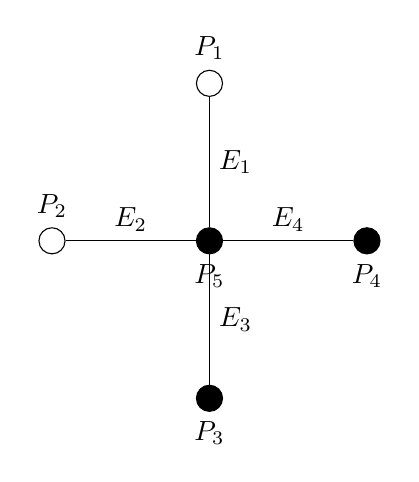
\begin{tikzpicture}
  \node (P1) at (0,2) [circle, draw, fill=white, label=above:$P_1$] {};
  \node (P2) at (-2,0) [circle, draw, fill=white, label=above:$P_2$] {};
  \node (P3) at (0,-2) [circle, draw, fill=black, label=below:$P_3$] {};
  \node (P4) at (2,0) [circle, draw, fill=black, label=below:$P_4$] {};
  \node (P5) at (0,0) [circle, draw, fill=black, label=below:$P_5$] {};
  \draw (P1) -- (P5) node[midway, right] {$E_1$};
  \draw (P2) -- (P5) node[midway, above] {$E_2$};
  \draw (P3) -- (P5) node[midway, right] {$E_3$};
  \draw (P4) -- (P5) node[midway, above] {$E_4$};
\end{tikzpicture}
\end{subcaptionblock}\hfill
\begin{subcaptionblock}{0.4\linewidth}
\centering
\subcaption{図2}
\begin{tikzpicture}
\node (P1') at (0,0) [circle, draw, fill=white, label=above:$P_1$] {};
\node (P1) at (2, 2.5) [circle, draw=none, fill=none, opacity=0] {};
\node (P2) at (-2, -2.5) [circle, draw=none, fill=none, opacity=0] {};
\end{tikzpicture}
\end{subcaptionblock}

% Fig. 3
\begin{subcaptionblock}{0.4\linewidth}
\subcaption{図3}
\centering
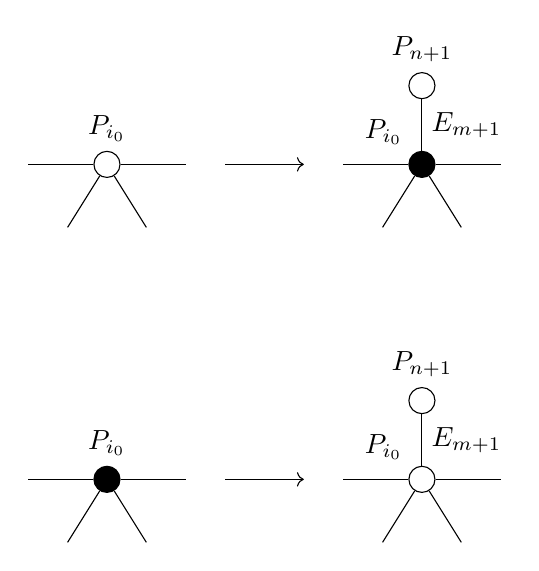
\begin{tikzpicture}
  % top left
  \node (p_i0) at (0,0) [circle, draw, fill=white, label=above:$P_{i_0}$] {};
  % P_{i0} から伸びる4本の線
  \draw (p_i0) -- (-1.0,0.0);
  \draw (p_i0) -- (1.0,0.0);
  \draw (p_i0) -- (-0.5,-0.8);
  \draw (p_i0) -- (0.5,-0.8);
  \draw[->] (1.5,0)--(2.5,0);

  % top right
  \node (p_i02) at (4,0) [circle, draw, fill=black, label=above left:$P_{i_0}$] {};
  \node (p_in)  at (4,1) [circle, draw, fill=white, label=above:$P_{n+1}$] {};
  % P_{i0} から伸びる4本の線
  \draw (p_i02) -- (3.0,0.0);
  \draw (p_i02) -- (5.0,0.0);
  \draw (p_i02) -- (3.5,-0.8);
  \draw (p_i02) -- (4.5,-0.8);
  \draw (p_i02) -- (p_in) node[midway, right] {$E_{m+1}$};

  % bottom left
  \node (p_i0) at (0,-4) [circle, draw, fill=black, label=above:$P_{i_0}$] {};
  % P_{i0} から伸びる4本の線
  \draw (p_i0) -- (-1.0,-4.0);
  \draw (p_i0) -- (1.0,-4.0);
  \draw (p_i0) -- (-0.5,-4.8);
  \draw (p_i0) -- (0.5,-4.8);
  \draw[->] (1.5,-4)--(2.5,-4);

  % bottom right
  \node (p_i02) at (4,-4) [circle, draw, fill=white, label=above left:$P_{i_0}$] {};
  \node (p_in)  at (4,-3) [circle, draw, fill=white, label=above:$P_{n+1}$] {};
  % P_{i0} から伸びる4本の線
  \draw (p_i02) -- (3.0,-4.0);
  \draw (p_i02) -- (5.0,-4.0);
  \draw (p_i02) -- (3.5,-4.8);
  \draw (p_i02) -- (4.5,-4.8);
  \draw (p_i02) -- (p_in) node[midway, right] {$E_{m+1}$};
\end{tikzpicture}
\end{subcaptionblock}\hfill
% Fig. 4
\begin{subcaptionblock}{0.4\linewidth}
\subcaption{図4}
\centering
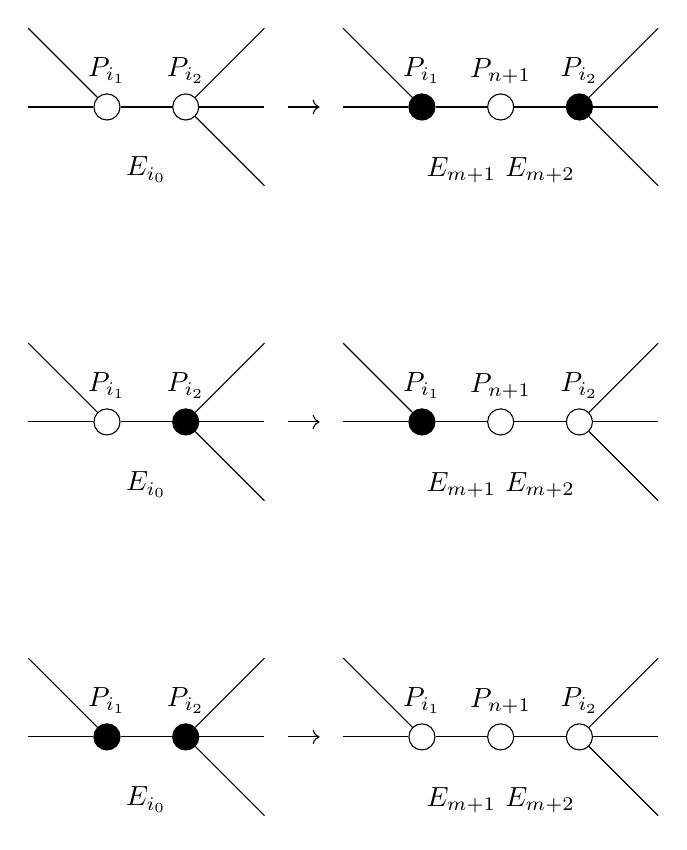
\begin{tikzpicture}
  % 左上の図
  \node (p_i1_top_left)  at (0,0) [circle, draw, fill=white, label=above:$P_{i_1}$] {};
  \node (p_i2_top_left)  at (1,0) [circle, draw, fill=white, label=above:$P_{i_2}$] {};
  \draw (p_i1_top_left) -- (p_i2_top_left);
  \draw (p_i1_top_left) -- (-1,0);
  \draw (p_i1_top_left) -- (-1,1);
  \draw (p_i2_top_left) -- (2,0);
  \draw (p_i2_top_left) -- (2,1);
  \draw (p_i2_top_left) -- (2,-1);
  \node at (0.5,-0.8) {$E_{i_0}$};
  \draw[->] (2.3,0)--(2.7,0);

  % 右上の図
  \node (p_i1_top_right)  at (4,0) [circle, draw, fill=black, label=above:$P_{i_1}$] {};
  \node (p_n_top_right)   at (5,0) [circle, draw, fill=white, label=above:$P_{n+1}$] {};
  \node (p_i2_top_right)  at (6,0) [circle, draw, fill=black, label=above:$P_{i_2}$] {};
  \draw (p_i1_top_right) -- (p_n_top_right);
  \draw (p_n_top_right) -- (p_i2_top_right);
  \draw (p_i1_top_right) -- (3,0);
  \draw (p_i1_top_right) -- (3,1);
  \draw (p_i2_top_right) -- (7,0);
  \draw (p_i2_top_right) -- (7,1);
  \draw (p_i2_top_right) -- (7,-1);
  \node at (4.5,-0.8) {$E_{m+1}$};
  \node at (5.5,-0.8) {$E_{m+2}$};

  % 左上の図
  \node (p_i1_top_left)  at (0,-4) [circle, draw, fill=white, label=above:$P_{i_1}$] {};
  \node (p_i2_top_left)  at (1,-4) [circle, draw, fill=black, label=above:$P_{i_2}$] {};
  \draw (p_i1_top_left) -- (p_i2_top_left);
  \draw (p_i1_top_left) -- (-1,-4);
  \draw (p_i1_top_left) -- (-1,-3);
  \draw (p_i2_top_left) -- (2,-4);
  \draw (p_i2_top_left) -- (2,-3);
  \draw (p_i2_top_left) -- (2,-5);
  \node at (0.5,-4.8) {$E_{i_0}$};
  \draw[->] (2.3,-4)--(2.7,-4);

  % 右上の図
  \node (p_i1_top_right)  at (4,-4) [circle, draw, fill=black, label=above:$P_{i_1}$] {};
  \node (p_n_top_right)   at (5,-4) [circle, draw, fill=white, label=above:$P_{n+1}$] {};
  \node (p_i2_top_right)  at (6,-4) [circle, draw, fill=white, label=above:$P_{i_2}$] {};
  \draw (p_i1_top_right) -- (p_n_top_right);
  \draw (p_n_top_right) -- (p_i2_top_right);
  \draw (p_i1_top_right) -- (3,-4);
  \draw (p_i1_top_right) -- (3,-3);
  \draw (p_i2_top_right) -- (7,-4);
  \draw (p_i2_top_right) -- (7,-3);
  \draw (p_i2_top_right) -- (7,-5);
  \node at (4.5,-4.8) {$E_{m+1}$};
  \node at (5.5,-4.8) {$E_{m+2}$};

  % 左上の図
  \node (p_i1_top_left)  at (0,-8) [circle, draw, fill=black, label=above:$P_{i_1}$] {};
  \node (p_i2_top_left)  at (1,-8) [circle, draw, fill=black, label=above:$P_{i_2}$] {};
  \draw (p_i1_top_left) -- (p_i2_top_left);
  \draw (p_i1_top_left) -- (-1,-8);
  \draw (p_i1_top_left) -- (-1,-7);
  \draw (p_i2_top_left) -- (2,-8);
  \draw (p_i2_top_left) -- (2,-7);
  \draw (p_i2_top_left) -- (2,-9);
  \node at (0.5,-8.8) {$E_{i_0}$};
  \draw[->] (2.3,-8)--(2.7,-8);

  % 右上の図
  \node (p_i1_top_right)  at (4,-8) [circle, draw, fill=white, label=above:$P_{i_1}$] {};
  \node (p_n_top_right)   at (5,-8) [circle, draw, fill=white, label=above:$P_{n+1}$] {};
  \node (p_i2_top_right)  at (6,-8) [circle, draw, fill=white, label=above:$P_{i_2}$] {};
  \draw (p_i1_top_right) -- (p_n_top_right);
  \draw (p_n_top_right) -- (p_i2_top_right);
  \draw (p_i1_top_right) -- (3,-8);
  \draw (p_i1_top_right) -- (3,-7);
  \draw (p_i2_top_right) -- (7,-8);
  \draw (p_i2_top_right) -- (7,-7);
  \draw (p_i2_top_right) -- (7,-9);
  \node at (4.5,-8.8) {$E_{m+1}$};
  \node at (5.5,-8.8) {$E_{m+2}$};

\end{tikzpicture}
\end{subcaptionblock}


% Fig. 5
\begin{subcaptionblock}{0.4\linewidth}
\subcaption{図5}
\centering
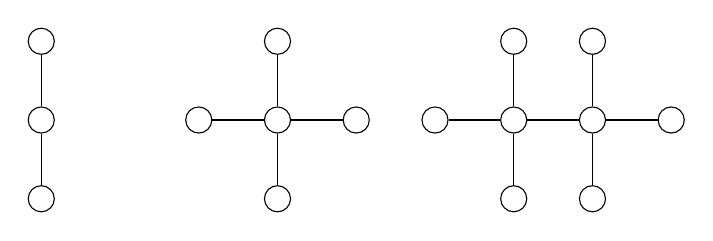
\begin{tikzpicture}
 \begin{scope}[shift={(0,0)}]
 \node  (P1) at (0,1) [circle, draw, fill=white] {};
  \node (P2) at (0,-1) [circle, draw, fill=white] {};
  \node (P3) at (0,0) [circle, draw, fill=white] {};
  \draw (P1) -- (P3);
  \draw (P2) -- (P3);
  \end{scope}

\begin{scope}[shift={(3,0)}]
  \node (P1) at (0,1) [circle, draw, fill=white] {};
  \node (P2) at (-1,0) [circle, draw, fill=white] {};
  \node (P3) at (0,-1) [circle, draw, fill=white] {};
  \node (P4) at (1,0) [circle, draw, fill=white] {};
  \node (P5) at (0,0) [circle, draw, fill=white] {};
  \draw (P1) -- (P5); 
  \draw (P2) -- (P5);
  \draw (P3) -- (P5);
  \draw (P4) -- (P5);
\end{scope}

\begin{scope}[shift={(6,0)}]
  \node (P1) at (0,1) [circle, draw, fill=white] {};
  \node (P2) at (-1,0) [circle, draw, fill=white] {};
  \node (P3) at (0,-1) [circle, draw, fill=white] {};
  \node (P4) at (1,0) [circle, draw, fill=white] {};
  \node (P5) at (0,0) [circle, draw, fill=white] {};
  \node (P6) at (1,1) [circle, draw, fill=white] {};
  \node (P7) at (1,-1) [circle, draw, fill=white] {};
  \node (P8) at (2,0) [circle, draw, fill=white] {};
  \draw (P1) -- (P5); 
  \draw (P2) -- (P5);
  \draw (P3) -- (P5);
  \draw (P4) -- (P5);
  \draw (P8) -- (P4);
  \draw (P7) -- (P4);
  \draw (P6) -- (P4);
\end{scope}
\end{tikzpicture}
\end{subcaptionblock}\hfill
\begin{subcaptionblock}{0.4\linewidth}
\subcaption{図6}
\centering
\begin{tikzpicture}
 \node (N1) at (0,0) [circle, draw, fill=white] {};
\node (N2) at (1,0) [circle, draw, fill=white] {};
\node (N3) at (2,0) [circle, draw, fill=white] {};
\node (dots) at (3,0) {$\dots$};
\node (Nn) at (4,0) [circle, draw, fill=white] {};
\draw (N1) -- (N2);
\draw (N2) -- (N3);
\draw (N3) -- (dots);
\draw (dots) -- (Nn);
\node (P1) at (2, 1.0) [circle, draw=none, fill=none, opacity=0] {};
\node (P2) at (-2, -1.0) [circle, draw=none, fill=none, opacity=0] {};
\end{tikzpicture}
\end{subcaptionblock}
\end{figure}


\end{document}